\begin{figure}[h!]
\centering

\begin{subfigure}{0.45\textwidth}
  \includegraphics[width=0.95\linewidth]{figures/het/het-r}
  \caption{Radial Cross Section at y=0}
  \label{fig:heta}
\end{subfigure}%
%
\begin{subfigure}{0.45\textwidth}
  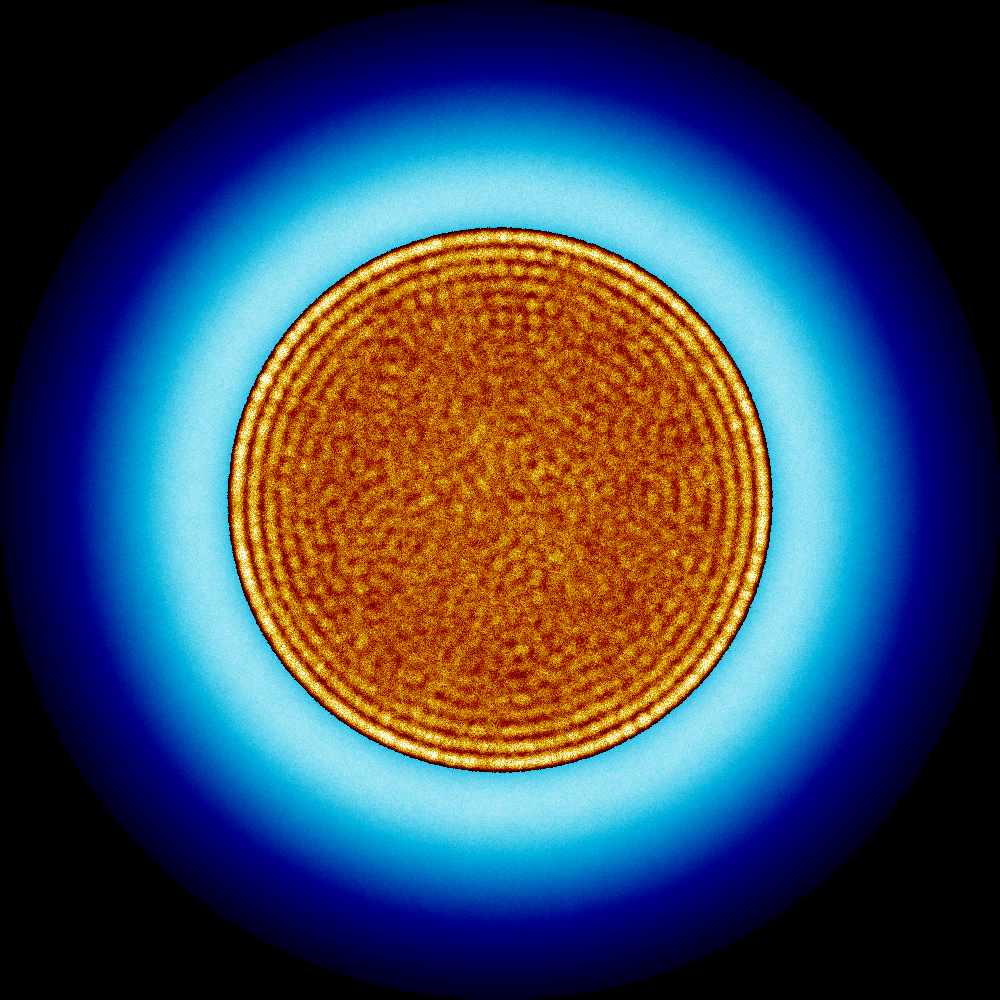
\includegraphics[width=0.95\linewidth]{figures/het/het-rm}
  \caption{Radial Mesh}
  \label{fig:hetb}
\end{subfigure}

\begin{subfigure}{0.45\textwidth}
  \includegraphics[width=0.95\linewidth]{figures/het/het-v}
  \caption{Axial Cross Section at z=0 }
  \label{fig:hetc}
\end{subfigure}
%
\begin{subfigure}{0.45\textwidth}
  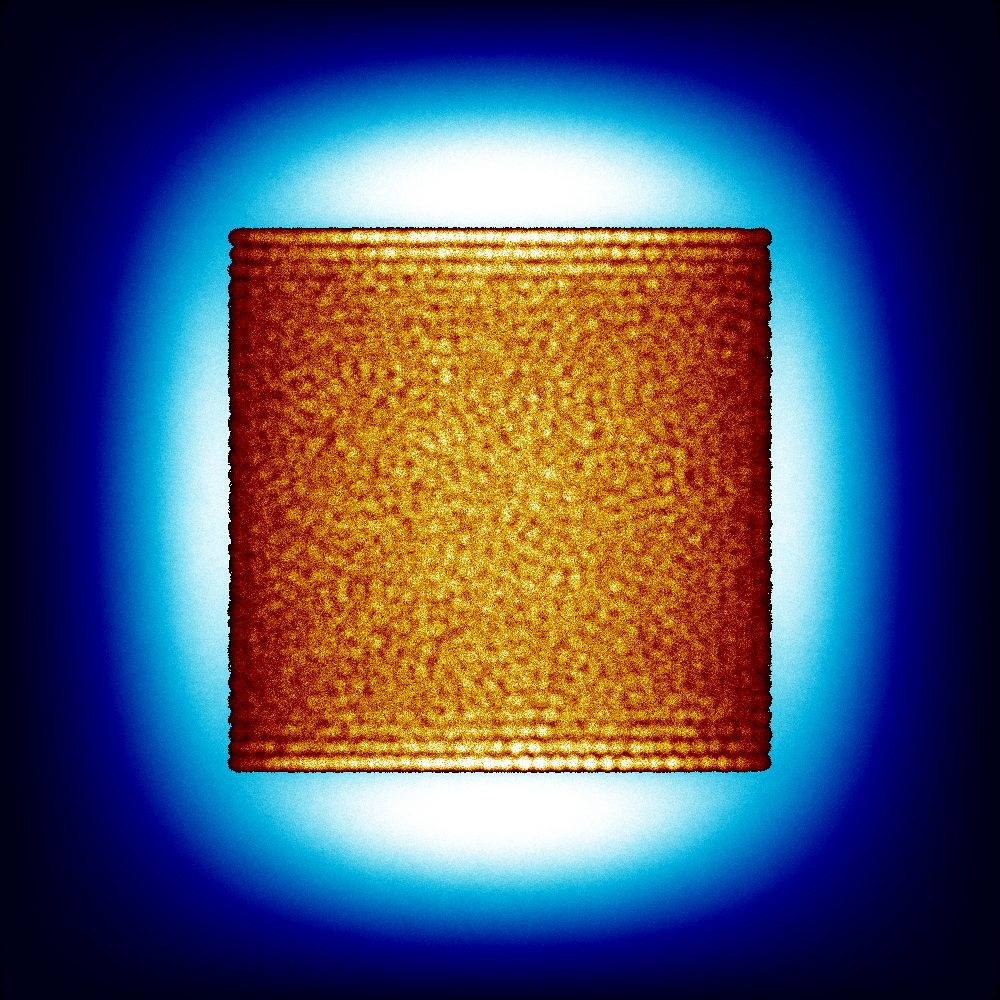
\includegraphics[width=0.95\linewidth]{figures/het/het-vm}
  \caption{Axial Mesh}
  \label{fig:hetd}
\end{subfigure}
%
\caption{Full Core Using Heterogenized Pebbles}
\label{fig:het}
\end{figure}